\documentclass[aspectratio=1610,xcolor=dvipsnames,t]{beamer} 

\usepackage{listings} 
\usepackage{color} 
\usepackage{xcolor}  
\usepackage{microtype} 
\usepackage{helvet} 
\usepackage{inconsolata} 
\usepackage[framemethod=TikZ]{mdframed} 
\usepackage{graphicx} 
\usepackage{alltt}
\usepackage{sverb} 
\usepackage{verbatim} 
\usepackage{pifont} 
\usepackage{alltt} 
\usepackage{helvet} 
\usepackage{algorithm}
\usepackage{algpseudocode}

\usetheme{Madrid} 
%\useoutertheme{smoothbars} 
\useinnertheme{rectangles} 

\setbeamertemplate{navigation symbols}{}
\setbeamertemplate{blocks}[default] 

%\definecolor{mypurple}{rgb}{.49,0,98}
%\setbeamercolor*{palette primary}{use=structure,fg=white,bg=green}
%\usecolortheme[rgb={0.9,0.2,0.2}]{structure}
%\usecolortheme[rgb={0.6,0.1,0.1}]{structure}

%\usecolortheme[rgb={0.2, 0.2, 0.8}]{structure} 
\usecolortheme[rgb={0.6, 0.0, 0.0}]{structure} 

\usepackage{color}
\definecolor{orange}{cmyk}{0,0.4,0.8,0.2}
\definecolor{darkorange}{rgb}{.71,0.21,0.01}
\definecolor{darkgreen}{rgb}{.12,.54,.11}
\definecolor{myteal}{rgb}{.26, .44, .56}
\definecolor{gray}{gray}{0.45}
\definecolor{lightgray}{gray}{.95}
\definecolor{mediumgray}{gray}{.8}
\definecolor{inputbackground}{rgb}{.95, .95, .85}
\definecolor{outputbackground}{rgb}{.95, .95, .95}
\definecolor{traceback}{rgb}{1, .95, .95}
\definecolor{inputbg}{rgb}{0.98, 0.98, 0.98}

\usepackage{listings} 
\lstset{language=c,
        %basicstyle=\footnotesize\ttfamily, 
        basicstyle=\small\ttfamily,
        columns=fullflexible, 
        %title=\lstname, 
        %numbers=left, stringstyle=\texttt, 
        %numberstyle={\tiny\texttt}, 
        keywordstyle=\color{blue}, 
        commentstyle=\color{darkgreen}, 
        stringstyle=\color{purple} } 


\mdfsetup{skipabove=\topskip, skipbelow=\topskip} 

\definecolor{codebg}{rgb}{0.99,0.99,0.99}

\global\mdfdefinestyle{code}{%
    frametitlerule=true,%
    frametitlefont=\small\bfseries\ttfamily,%
    frametitlebackgroundcolor=lightgray,%
    backgroundcolor=codebg,%
    linecolor=gray, linewidth=0.5pt,%
    leftmargin=0.5cm, rightmargin=0.5cm,%
    roundcorner=2pt,%
    innerleftmargin=5pt
}

\global\mdfdefinestyle{code2}{%
    topline=false,%
    bottomline=false,%
    leftline=true,%
    rightline=false,%
    backgroundcolor=codebg,%
    linecolor=gray, linewidth=0.5pt,%
    leftmargin=0.0cm, rightmargin=0.0cm,%
    innerleftmargin=1pt
}

\newcommand{\showcode}[1]{\begin{mdframed}[style=code] %
                            \lstinputlisting{#1}% 
                          \end{mdframed}% 
}


\title[BDI Concepts]{BDI Concepts and Agent Oriented Systems} 
\subtitle{Knowledge Representation and Reasoning} 
\author[Michael Papasimeon]{Michael Papasimeon \\[0.2cm] \tiny{Intelligent Agent Lab} } 
\date{22 October 2003} 

\begin{document}

\begin{frame}
    \maketitle
\end{frame} 

\begin{frame}{Outline} 
    \begin{itemize}
        \item The Intentional Stance
        \item Beliefs, Desires and Intentions
        \item Rational Agency and BDI
        \item Rao and Georgeff's Theoretical BDI Interpreter
        \item Wooldridge's Agent Control Loops
        \item dMARS and JACK
        \item BDI Agent Architecture
        \item Example dMARS Plan
        \item BDI Dynamics
        \item References
    \end{itemize} 
\end{frame} 

\begin{frame}{The Intentional Stance} 
    The philosopher Daniel Dennet proposed three ways (stances) at which
    we can predict things about the world:
    \begin{block}{Dennet's Stances} 
        \begin{itemize} 
            \item \textbf{Physical} Stance
            \item \textbf{Design} Stance
            \item \textbf{Intentional} Stance
        \end{itemize} 
    \end{block} 
\end{frame} 

\begin{frame}{Beliefs, Desires and Intentions} 
    Internal mental attitudes of a rational BDI agent (or mental state):
    \begin{block}{Beliefs} 
        What an agent believes about the world, itself and other agents
        (informational).
    \end{block} 
    \begin{block}{Desires} 
        What an agent want to achieve (motivational).
    \end{block} 
    \begin{block}{Intentions} 
        How the agent tries to achieve desires (deliberational).
    \end{block} 
\end{frame} 

\begin{frame}{Rational Agency and BDI} 
    \begin{description}
        \item[Daniel Dennet:] Folk Psychology
        \item[Michael Bratman:] Rational Agency
        \item[Rao and Georgeff:] Formal Logical Framework
        \item[Programming Languages:] PRS, dMARS, JACK, JAM, C-PRS, IRMA
    \end{description} 
\end{frame} 

\begin{frame}{Theoretical BDI Interpreter (Rao and Georgeff)} 
    \begin{block}{BDI Interpreter} 
        \showcode{raogeorgeff.py} 
    \end{block} 
\end{frame} 

\begin{frame}{Basic Agent Control Loop 1}
    \begin{block}{Adapted from Wooldridge...}
        \begin{algorithmic}[0]
            \Procedure{Agent Control Loop 1}{}
                \While{True}
                    \State $\texttt{observe-the-world();}$ 
                    \State $\texttt{update-internal-world-model();}$
                    \State $\texttt{deliberate-about-what-intention-to-achieve-next()}$
                    \State $\texttt{use-means-end-reasoning-to-get-a-plan-for-next-intention()}$
                    \State $\texttt{execute-the-plan}$
                \EndWhile
            \EndProcedure
        \end{algorithmic} 
    \end{block} 
\end{frame} 

\begin{frame}{Basic Agent Control Loop 2} 
    \begin{block}{Adapted from Wooldridge...} 
        \begin{algorithmic}[0] 
            \Procedure{Agent Control Loop 2}{$B_0$} 
                \State $B \gets B_0$
                \While{True} 
                    \State $\rho \gets \texttt{get\_next\_percept}();$
                    \State $B \gets \texttt{brf}(B, \rho);$
                    \State $D \gets \texttt{deliberate}(B);$ 
                    \State $\pi \gets \texttt{plan}(B, I); $
                    \State $\texttt{execute}(\pi); $
                \EndWhile
            \EndProcedure
        \end{algorithmic} 
    \end{block} 
\end{frame} 

\begin{frame}{Basic Agent Control Loop 3} 
    \begin{block}{Adapted from Wooldridge...} 
        \begin{algorithmic}[0] 
            \Procedure{Agent Control Loop 3}{$B_0, I_0$} 
                \State $B \gets B_0$
                \State $I \gets I_0$
                \While{True} 
                    \State $\rho \gets \texttt{get\_next\_percept}();$
                    \State $B \gets \texttt{brf}(B, \rho);$
                    \State $D \gets \texttt{options}(B I);$ 
                    \State $I \gets \texttt{filter}(B, D, I); $
                    \State $\pi \gets \texttt{plan}(B, I); $
                    \State $\texttt{execute}(\pi); $
                \EndWhile
            \EndProcedure
        \end{algorithmic} 
    \end{block} 
\end{frame} 

\begin{frame}{dMARS and JACK} 
    \begin{itemize} 
        \item Implementations of the BDI model
        \item Idea of plans as reciples (pre-planning) 
        \item Least commitment 
        \item Bounded rationality
        \item Dynamic environment
        \item Goals, beliefs, plans
        \item Intentions and run-time (not design time) constructs
    \end{itemize} 
\end{frame} 

\begin{frame}{A BDI Agent Architecture} 
    \begin{center} 
        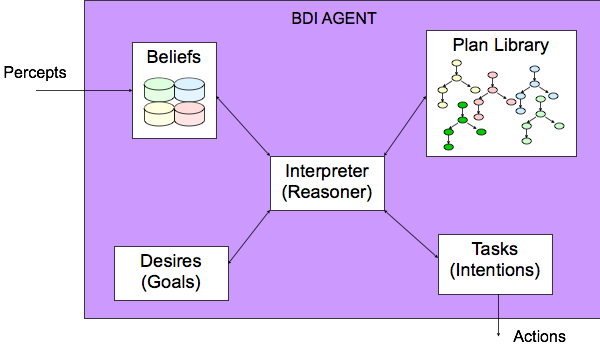
\includegraphics[width=0.7\textwidth]{reasoner} 
    \end{center} 
\end{frame} 

\begin{frame}{Example dMARS Plan} 
    \begin{center} 
        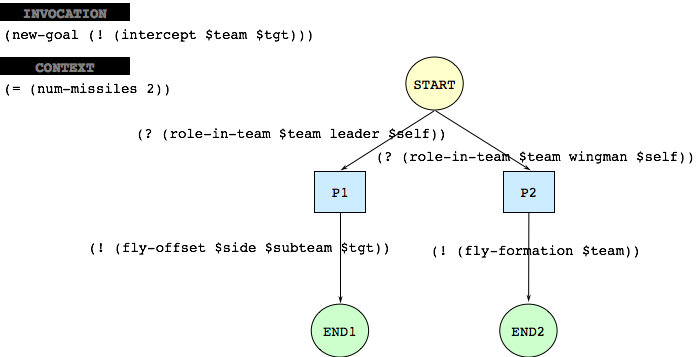
\includegraphics[width=0.8\textwidth]{dmars} 
    \end{center} 
\end{frame} 

\begin{frame}{BDI Dynamics (1)}
    \begin{enumerate}
        \item An event occurs.
            \begin{itemize} 
                \item A goal is posted (internal).
                \item A change in the environment and hence a change in 
                      belief (external). 
            \end{itemize} 
        \item Agent reasoner searches through the plan library to
              find the set of plans which can handle this event
              (defined by the invocation condition).
        \item This may result in in 10 plans out of 500 which can
              handle the event. Out of these 10 plans, the agent
              reasoner then chooses only those which are 
              appropriate for this \textbf{context} -- that is, 
              the current situation. 
    \end{enumerate} 
\end{frame} 

\begin{frame}{BDI Dynamics (2)}
    \begin{enumerate}
        \setcounter{enumi}{4}
        \item This may result in 6 plans out of the 10 which are
              \textbf{applicable} in this context. 
        \item The agent then chooses one of the plans, puts it on the
              \textbf{intention stack}, and starts executing the plan
              steps in the plan.
        \item This executing plan is called an \textbf{intention} to 
              achieve the original \textbf{goal}. 
        \item If the plan fails, the agent will try on of the other
              applicable plans until one of them succeeds in 
              achieving the goal or all of them fail, in which case
              the goal will fail.
    \end{enumerate} 
\end{frame} 

\begin{frame}{BDI Dynamics Notes}
    \begin{itemize} 
        \item It is possible to determine which plan is chosen in the
              applicable plan set by using \textbf{meta-level reasoning}.
        \item Plans can wait until particular beliefs are satisfied.
        \item Plan steps can involve trying to achieve \textbf{sub-goals}.
        \item When trying to achieve a sub-goal, the existing plan
              is suspended and the new plan is put on top of the
              \textbf{intention stack}. 
    \end{itemize} 
\end{frame} 

\begin{frame}{References}
    \begin{itemize} 
        \item \emph{Reasoning About Rational Agents}, Michael Wooldridge
        \item \emph{The Intentional Stance}, Daniel Dennet
        \item \emph{BDI Agents: From Theory to Practice},  
Anand Rao and Michael Georgeff
        \item \emph{Modeling Rational Agents within a BDI-Architecture}, Anand Rao 
              and Michael Georgeff
    \end{itemize} 
\end{frame} 
\end{document}
